% loopmarket — a 30-minute introduction for a Swarm audience
% Build: make            (figures first, then the deck)
\documentclass[aspectratio=169,11pt]{beamer}
% Shared style for every figure and for the deck: one accent, one
% highlight, thin lines, rounded nodes, nothing decorative.
\usepackage[T1]{fontenc}
\usepackage{lmodern}
\renewcommand{\familydefault}{\sfdefault}
\usepackage{tikz}
\usetikzlibrary{arrows.meta,positioning,calc,shapes.misc,fit,backgrounds,decorations.pathreplacing}
\definecolor{ink}{RGB}{40,40,40}
\definecolor{soft}{RGB}{150,150,150}
\definecolor{faint}{RGB}{225,225,225}
\definecolor{accent}{RGB}{0,95,115}
\definecolor{accentlight}{RGB}{214,232,236}
\definecolor{warn}{RGB}{196,84,40}
\definecolor{warnlight}{RGB}{247,226,216}
\tikzset{
  every picture/.style={color=ink, line width=0.5pt, font=\small},
  node distance=12mm and 18mm,
  box/.style={draw=ink, rounded corners=2pt, fill=white, inner sep=5pt, minimum height=7mm, align=center},
  maker/.style={box, minimum width=18mm},
  cat/.style={box, inner sep=3.5pt, minimum height=6mm},
  root/.style={box, fill=accentlight, draw=accent},
  bad/.style={box, fill=warnlight, draw=warn},
  ghost/.style={box, draw=soft, text=soft, dashed},
  flow/.style={-{Stealth[length=4pt,width=3.5pt]}, line width=0.5pt},
  sub/.style={-{Stealth[length=4pt,width=3.5pt]}, line width=0.5pt, color=soft},
  strong/.style={flow, color=accent, line width=0.8pt},
  wrong/.style={flow, color=warn},
  lbl/.style={font=\footnotesize, text=ink, inner sep=1.5pt, fill=white},
  note/.style={font=\footnotesize, text=soft, align=center},
  rate/.style={font=\footnotesize, text=accent, inner sep=1pt, fill=white},
}

\usepackage{booktabs}
\usepackage{amsmath}
\usepackage{graphicx}
\graphicspath{{figures/}}

% --- a quiet theme -----------------------------------------------------------
\usetheme{default}
\usefonttheme{professionalfonts}
\setbeamertemplate{navigation symbols}{}
\setbeamercolor{normal text}{fg=ink}
\setbeamercolor{structure}{fg=accent}
\setbeamercolor{frametitle}{fg=ink}
\setbeamercolor{title}{fg=ink}
\setbeamercolor{alerted text}{fg=warn}
\setbeamerfont{frametitle}{size=\large, series=\bfseries}
\setbeamerfont{title}{size=\LARGE, series=\bfseries}
\setbeamerfont{subtitle}{size=\normalsize, series=\mdseries}
\setbeamertemplate{frametitle}{\vspace*{6mm}\insertframetitle\par\vspace*{1mm}}
\setbeamertemplate{itemize items}{\textcolor{accent}{\raisebox{0.35ex}{\rule{0.9ex}{0.9ex}}}}
\setbeamertemplate{itemize subitem}{\textcolor{soft}{--}}
\setbeamertemplate{footline}{%
  \hfill\textcolor{soft}{\footnotesize\insertframenumber}\hspace*{6mm}\vspace*{3mm}}
\setlength{\leftmargini}{1.4em}
\setbeamersize{text margin left=10mm, text margin right=10mm}
\newcommand{\src}[1]{{\footnotesize\textcolor{soft}{#1}}}
\newcommand{\fig}[2][0.9]{\centering\includegraphics[width=#1\linewidth, height=0.7\textheight, keepaspectratio]{#2}}
\newcommand{\colfig}[2][0.78]{\includegraphics[width=\linewidth, height=#1\textheight, keepaspectratio]{#2}}

\title{Markets without a platform}
\subtitle{the loop economy on Swarm}
\author{Peter F\"oldi\'ak}
\date{September 2026}

\begin{document}

\begin{frame}[plain]
  \vspace*{18mm}
  {\usebeamerfont{title}\usebeamercolor[fg]{title}\inserttitle\par}
  \vspace{3mm}
  {\usebeamerfont{subtitle}\insertsubtitle\par}
  \vspace{12mm}
  {\small\insertauthor\qquad\textcolor{soft}{\insertdate}\par}
  \vspace{2mm}
  {\small\textcolor{soft}{loopmarket $\cdot$ ontodag $\cdot$ recordstore $\cdot$ factbond \quad github.com/petfold}\par}
\end{frame}

% =============================================================== Part 1
\begin{frame}{Two failure modes, one cause}
  \fig[0.95]{fig-commerce}
  \vspace{2mm}
  \begin{itemize}
    \item Either the market is somebody's property, or there is no market at all.
    \item Missing piece: a \emph{shared, unowned} market structure.
  \end{itemize}
\end{frame}

\begin{frame}{The rent, the gate, the ranking}
  \begin{itemize}
    \item Take rates: app stores $\sim$30\%; marketplaces 15\%+ referral, plus logistics and ads. \src{[verify]}
    \item Gatekeeping: delisting is unilateral and unappealable.
    \item Ranking: the platform's algorithm decides who exists.
  \end{itemize}
  \vspace{4mm}
  Platform power is structural: whoever holds the only index can charge for inclusion and shape the market by \alert{omission}.
\end{frame}

\begin{frame}{The deeper limit: everything must pass through money}
  \begin{columns}[T]
    \begin{column}{0.5\textwidth}
      \begin{itemize}
        \item Trade needs a double coincidence of wants, or a common medium.
        \item Where the medium is thin, good trades don't happen.
        \item Time banks stall in every town: within one service type the web of offers is too sparse to close cycles.
      \end{itemize}
    \end{column}
    \begin{column}{0.5\textwidth}
      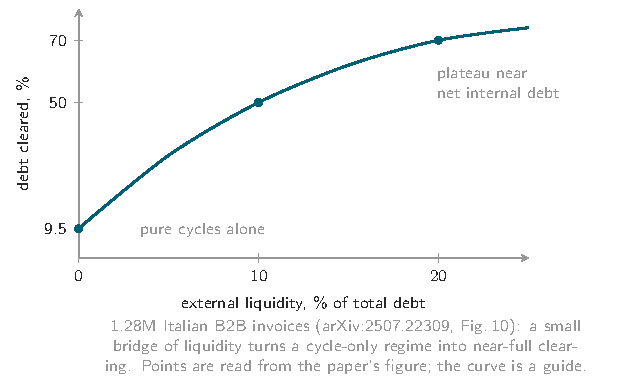
\includegraphics[width=\linewidth]{fig-liquidity}
    \end{column}
  \end{columns}
\end{frame}

% =============================================================== Part 2
\begin{frame}{One uniform offer}
  \begin{columns}[T]
    \begin{column}{0.55\textwidth}
      \colfig{fig-offer}
    \end{column}
    \begin{column}{0.45\textwidth}
      \vspace{6mm}
      \begin{itemize}
        \item A thing, a time, a place, a validity, a price.
        \item Give or want: the same form.
        \item Priced on the maker's \emph{own scale}: nothing is held or transferred; the numbers cancel inside a loop.
        \item A shop, a person, a bus with empty seats, a stablecoin: all makers.
      \end{itemize}
    \end{column}
  \end{columns}
\end{frame}

\begin{frame}{The simplest loop}
  \fig[0.7]{fig-loop2}
\end{frame}

\begin{frame}{The simplest loop, on two scales}
  \fig[0.85]{fig-loop2-scales}
\end{frame}

\begin{frame}{The catalogue: meanings, minutes and map cells, one order}
  \fig[0.95]{fig-ontodag}
\end{frame}

\begin{frame}{ontodag as the language of offers}
  \begin{columns}[T]
    \begin{column}{0.55\textwidth}
      \colfig[0.62]{fig-ontodag-match}
    \end{column}
    \begin{column}{0.45\textwidth}
      \vspace{4mm}
      \begin{itemize}
        \item One primitive: intersection of descendant cones.
        \item Shipped this week: the \texttt{core} pack, 4,137 consensus categories (WordNet, SUMO, OpenCyc, Wikidata, schema.org as witnesses) + ten domain packs.
        \item A catalogue is a \emph{pinned root}: every offer names the version it was written against.
        \item Honest footnote: goods are rich (toaster, jeans, tomato); services are the next pack.
      \end{itemize}
    \end{column}
  \end{columns}
\end{frame}

\begin{frame}{Fits-within, three ways}
  \fig[0.95]{fig-fitswithin}
\end{frame}

\begin{frame}{Loops: the trade nobody asked for}
  \begin{columns}[T]
    \begin{column}{0.5\textwidth}
      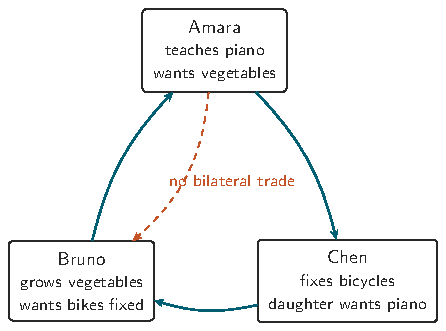
\includegraphics[width=\linewidth]{fig-triangle-wants}
    \end{column}
    \begin{column}{0.5\textwidth}
      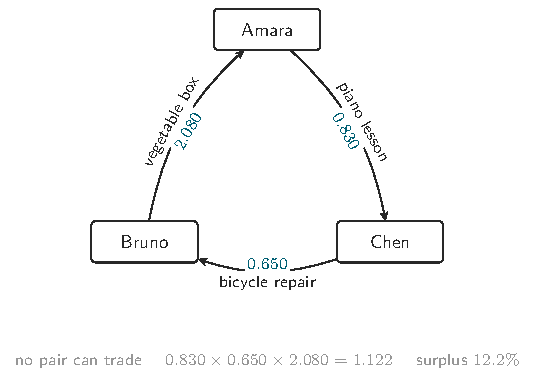
\includegraphics[width=\linewidth]{fig-loop3}
    \end{column}
  \end{columns}
\end{frame}

\begin{frame}{A profitable loop is a negative cycle}
  \fig[0.8]{fig-neglog}
\end{frame}

\begin{frame}{Settlement trusts no one}
  \fig[0.9]{fig-settlement}
\end{frame}

\begin{frame}{Money is just another offer}
  \fig[0.8]{fig-bridge}
\end{frame}

% =============================================================== Part 3
\begin{frame}{The stack, and why it is Swarm-shaped}
  \begin{columns}[T]
    \begin{column}{0.55\textwidth}
      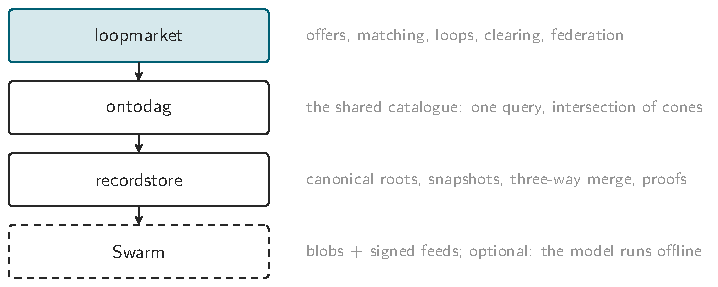
\includegraphics[width=\linewidth]{fig-stack}
    \end{column}
    \begin{column}{0.45\textwidth}
      \vspace{2mm}
      \begin{itemize}
        \item Book = versioned keyspace, canonical roots: equal content $\Rightarrow$ equal reference.
        \item One book per maker, under the maker's own feed and signer. Identity \emph{is} the feed owner.
        \item Everything so far runs on a \emph{light} node.
        \item Postage TTL is the offer's lifetime; withdrawal is a tombstone, never a delete.
      \end{itemize}
    \end{column}
  \end{columns}
\end{frame}

\begin{frame}{A maker's book is a feed}
  \fig[0.75]{fig-feed}
\end{frame}

\begin{frame}{Invariants the tests refuse to let you break}
  \begin{columns}[T]
    \begin{column}{0.5\textwidth}
      \begin{itemize}
        \item[U1] uniform offer form
        \item[U2] immutable, content-addressed
        \item[U3] settlement trusts no solver
        \item[U4] solve against pinned roots
      \end{itemize}
    \end{column}
    \begin{column}{0.5\textwidth}
      \begin{itemize}
        \item[U5] positive rates only
        \item[U6] deterministic baseline solver
        \item[U7] vocabulary fails closed
        \item[U11] no partially-filled loop survives a merge
      \end{itemize}
    \end{column}
  \end{columns}
  \vspace{4mm}
  \centering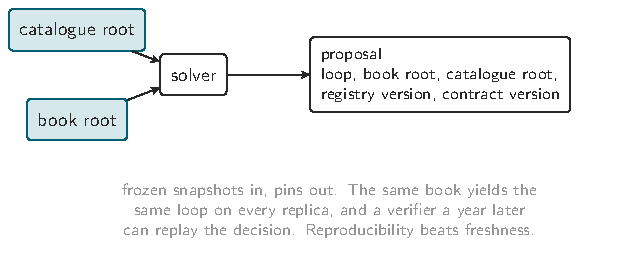
\includegraphics[width=0.8\linewidth, height=0.36\textheight, keepaspectratio]{fig-pins}
\end{frame}

\begin{frame}{The federated book}
  \fig[0.95]{fig-federation}
\end{frame}

\begin{frame}{Demo: three feeds, two honest aggregators, one censor}
  \begin{itemize}
    \item Three makers publish under their own feeds; two aggregators fold in different orders: byte-identical manifests.
    \item Mallory forges an offer in Amara's name: refused at the fold, with an attributed reason.
    \item Bruno withdraws: a tombstone that survives merges.
    \item Cain announces Chen's book and silently drops it.
    \item Settlement bases its own book on the fold; the loop settles; a follower reads six atomic fills from the manifest alone.
  \end{itemize}
  \vspace{3mm}
  \src{\texttt{examples/demo\_federation.py} -- in memory $\sim$5\,s; live on a Bee light node 2--7 min (recording).}
\end{frame}

\begin{frame}{Omission is a proof, not a suspicion}
  \fig[0.95]{fig-cain}
\end{frame}

\begin{frame}{Are aggregators necessary?}
  \begin{itemize}
    \item Not for correctness, trust or permission: the fold is pure; any reader recomputes it.
    \item For read cost: a feed lookup costs seconds; a solver folding 1,000 maker feeds pays 1,000 lookups per beat.
    \item Direction: solver-side folding is the default; manifests are disposable caches.
    \item Discovery via a public log (Gnosis registry events as the floor, GSOC as the fast path), never via a party who can omit.
  \end{itemize}
  \vspace{4mm}
  \textbf{Question for this room:} GSOC reception from light nodes, and pub/sub. Content-routed GSOC (one address per catalogue cone $\times$ geo cell $\times$ day) would make the index \emph{the address space}. Stamps are not the problem; delivery guarantees are.
\end{frame}

\begin{frame}{Roadmap}
  \fig[0.95]{fig-roadmap}
  \vspace{4mm}
  The one point of trust today is settlement. P2 removes it: inclusion and absence under the pinned book root, verified on Gnosis with recordstore's canonical-trie proofs.
\end{frame}

% =============================================================== Part 4
\begin{frame}{Swarm AI Data Exchange and loopmarket: same substrate, same idioms}
  \begin{itemize}
    \item Both: content-addressed catalogues on Swarm; an atomic root in a feed; feed owner as identity; a light node suffices to read.
    \item Exchange: Agent Card (ERC-8004) $\to$ catalog feed $\to$ Mantaray root $\to$ \texttt{item.jsonld}; ACT-encrypted content; x402 purchase endpoint.
    \item loopmarket: per-maker feed $\to$ recordstore root $\to$ offers; aggregator manifests; settlement feed.
  \end{itemize}
  \vspace{4mm}
  What the exchange got right and shipped: ACT per purchase, schema.org-first vocabulary, server minimization as a principle, a working purchase flow.
\end{frame}

\begin{frame}{A storefront and a clearing house}
  \fig[0.95]{fig-exchange-vs-loop}
\end{frame}

\begin{frame}{The differences}
  \footnotesize
  \renewcommand{\arraystretch}{1.25}
  \begin{tabular}{@{}p{20mm}p{54mm}p{58mm}@{}}
    \toprule
    & Swarm AI Data Exchange & loopmarket \\
    \midrule
    trade shape & bilateral: one publisher, one buyer, one item & multilateral loops; no pair needs to want each other \\
    price & set by the publisher, in a stablecoin & discovered; each maker on their own scale; surplus when $\prod$ rates $>1$ \\
    medium & required (stablecoin via x402) & none required; money is a bridge offer \\
    described & data assets (schema.org + \texttt{swarm-cat:}) & anything: catalogue conjunction $\times$ time $\times$ place \\
    required server & the publisher's x402 endpoint & none for makers; settlement only (on chain in P2) \\
    trust & ERC-8004 reputation + facilitator & re-verification; bonds where verification fails; reputation derived, never a gate \\
    privacy & ACT per purchase & none yet (P4) \\
    maturity & working purchase flow & prototype; live on Swarm; mock settlement \\
    \bottomrule
  \end{tabular}
\end{frame}

\begin{frame}{Why not reputation-based}
  \begin{itemize}
    \item eBay: 0.3\% of transactions rated negative, yet $P(\text{negative} \mid \text{partner rated negative}) > 37\%$: retaliation suppressed truthful feedback until one-sided ratings in 2007. \src{Resnick \& Zeckhauser}
    \item Cheap ratings inflate toward uselessness. \src{Filippas, Horton, Golden, EC'18}
    \item loopmarket's rule U12: standing counts settled, fee-paid loops only; loss experience comes from bonded, adjudicated events (factbond).
  \end{itemize}
  \vspace{4mm}
  Reputation answers ``should I trust this seller''. loopmarket makes the question unnecessary where it can, and expensive to game where it cannot. Reputation becomes a statistic you derive, not an institution you believe.
\end{frame}

\begin{frame}{x402 and ERC-8004 fit: as legs, identities and proofs}
  \begin{itemize}
    \item \textbf{x402} is a bilateral rail; it cannot settle a $k$-leg loop. It fits three places the plan already has: the stablecoin leg of a bridge offer (settlement cargo, never the scoring numeraire); paid aggregator \emph{serving}, never inclusion; solver fee collection.
    \item \textbf{ERC-8004 identity}: an Agent Card service entry naming the maker's book feed owner is exactly the announcement channel, with the chain registry as the censorship-resistant floor.
    \item \textbf{ERC-8004 reputation}: publish one-sided, aggregated signals derived from settled loops; consume feedback as one input to risk premia; never gate a trade on it.
    \item \textbf{ERC-8004 validation}: settlement receipts and factbond certificates are validation events with proofs.
  \end{itemize}
  \vspace{2mm}
  x402 for the money leg, loopmarket for the parts x402 cannot see.
\end{frame}

\begin{frame}{How we could converge}
  \fig[0.95]{fig-convergence}
\end{frame}

\begin{frame}{How we could converge}
  \begin{enumerate}
    \item One ERC-8004 Agent Card carrying both a \texttt{swarm-ai-catalog} and a \texttt{loopmarket-book} service.
    \item Bridge adapter: every catalog item is a give offer priced in a stablecoin; publish the catalog into a book unchanged.
    \item The x402 endpoint as a fulfilment oracle: an ACT grant is a verifiable proof of delivery.
    \item Shared vocabulary: the exchange's schema.org/\texttt{swarm-cat:} terms as an ontodag pack.
    \item Discovery as a public log, not an indexer: keep ``no synthesized server views'', add ``no party who can omit''.
    \item Keep the one-currency assumption out of the data model: a price is a number on \emph{some} scale.
  \end{enumerate}
  \vspace{1mm}
  In return: ACT as a P4 Tier-1 candidate, x402 pragmatism, ERC-8004 identity, and the habit of shipping.
\end{frame}

% =============================================================== Close
\begin{frame}{Asks to the room}
  \begin{itemize}
    \item GSOC reception from light nodes; pub/sub timing.
    \item A services layer for ontodag's core pack: the goods are in; repair, tutoring, cleaning are not.
    \item A first vertical: digital services, agents first.
  \end{itemize}
  \vspace{8mm}
  The root is the market. Swarm holds the books. The chain is the floor for discovery. The one remaining point of trust is settlement, and it is next.
  \vspace{6mm}
  \src{github.com/petfold: loopmarket, ontodag, recordstore, factbond}
\end{frame}

% =============================================================== Backup
\appendix
\begin{frame}{Backup: a match is an edge}
  \fig[0.9]{fig-match}
\end{frame}
\begin{frame}{Backup: Graphviz renderings (dot2tex)}
  \begin{columns}[T]
    \begin{column}{0.33\textwidth}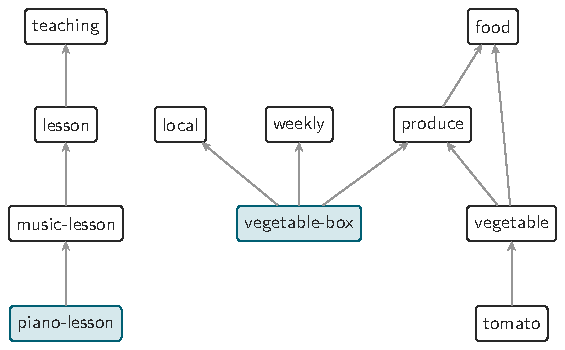
\includegraphics[width=\linewidth]{dot-ontodag}\end{column}
    \begin{column}{0.33\textwidth}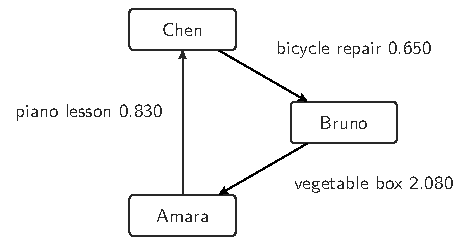
\includegraphics[width=\linewidth]{dot-loop3}\end{column}
    \begin{column}{0.33\textwidth}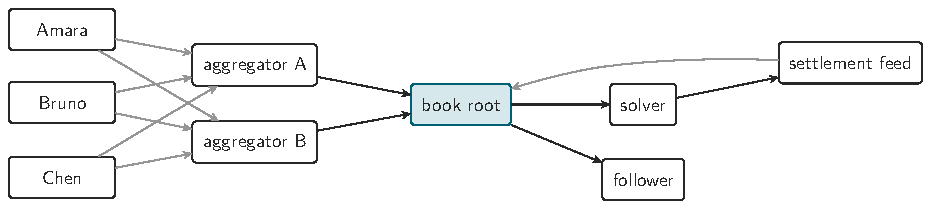
\includegraphics[width=\linewidth]{dot-federation}\end{column}
  \end{columns}
\end{frame}
\end{document}
